% Bu dosya hem bağımsız hem de 00_kitap.tex içinden derlenebilir.
% Ana kitapta: \begin{refsection}\subfile{05nciBolum.tex}\printbib\end{refsection}
\documentclass[00_kitap.tex]{subfiles}

\begin{document}
\BolumKaynakcaBaslat

\setcounter{section}{4}
\section{Dalga Mekaniğinin Genel Yapısı}
\label{sec:dalga_mekanigi_genel}

Önceki bölümlerde belirli potansiyeller altında Schrödinger denklemini
çözerek enerji özdeğerlerini ve bunlara karşılık gelen özfonksiyonları
bulduk. Bu bölümde bu özel örnekleri hatırlayarak daha genel bir yapı
kuracağız. Bu doğrultuda özfonksiyonları ve açılım teoremini, fiziksel
gözlenebilirleri temsil eden işlemcileri, Hermitliği, dejenereliği ve
beklenen değerlerin zamana bağlılığını inceleyeceğiz. Son olarak kuantum
hareket denklemleri ile klasik mekanik arasındaki ilişkiyi ele alacağız
\cite{book:Gasiorowicz}.

Anlatımı sade tutmak için öncelikle bir boyutta hareket eden, spin
serbestlik derecesini açıkça içermeyen tek bir parçacıkla çalışacağız.
Bu sistemin saf durumunun $\Psi(x,t)$ dalga fonksiyonuyla tanımlandığını
ve bu fonksiyonun durum hakkında elde edilebilecek bilgiyi içerdiğini
kabul ediyoruz.

% Kaynak PDF s. 1--6.
\subsection{Özfonksiyonlar ve Özdeğerler}
\label{sec:05_ozfonksiyonlar}

\subsubsection{Hamiltonyen işlemcisi}

Dalga fonksiyonunun zamanla değişimini zamana bağlı Schrödinger
denklemi belirler:
\begin{equation}
 i\hbar\frac{\partial\Psi(x,t)}{\partial t}=\hat H\Psi(x,t).
 \label{eq:05_sch_zaman}
\end{equation}
Burada $\hat H$ Hamiltonyen işlemcisidir. Relativistik olmayan bir
parçacık, konuma bağlı bir skaler potansiyel etkisindeyse,
\begin{equation}
 \hat H=\frac{\hat p^2}{2m}+\hat V,
 \qquad
 \hat p=-i\hbar\frac{\partial}{\partial x},
 \qquad (\hat V\Psi)(x,t)=V(x)\Psi(x,t)
 \label{eq:05_hamiltonyen}
\end{equation}
yazılır. Dolayısıyla konum gösteriminde,
\begin{equation}
 \hat H=-\frac{\hbar^2}{2m}\frac{\partial^2}{\partial x^2}+V(x)
\end{equation}
biçimindedir. Bu bölümde aksi söylenmedikçe potansiyelin zamana açıkça
bağlı olmadığını kabul edeceğiz.

Bu durumda değişkenlerine ayrılmış özel çözümler,
\begin{equation}
 \Psi_E(x,t)=u_E(x)e^{-iEt/\hbar}
 \label{eq:05_duragan}
\end{equation}
şeklinde yazılabilir. Denk.~\eqref{eq:05_sch_zaman}'da yerine
konulduğunda uzaysal fonksiyon için,
\begin{equation}
 \boxed{\hat H u_E(x)=E u_E(x)}
 \label{eq:05_enerji_ozdeger}
\end{equation}
elde edilir. Hamiltonyenin etkisiyle yalnızca sabit bir çarpanla
değişen $u_E$ fonksiyonuna \emph{özfonksiyon}, bu çarpan olan $E$'ye
\emph{özdeğer} denir. Fiziksel sınır şartlarını sağlayan çözümler,
sistemin izinli enerji değerlerini belirler.

\subsubsection{Diklik, normalizasyon ve tamlık}

Önceki örneklerden tanıdığımız özellikleri topluca hatırlayalım.
Hermit bir Hamiltonyenin farklı enerji özdeğerlerine karşılık gelen
özfonksiyonları diktir:
\begin{equation}
 E_n\ne E_j\quad\Longrightarrow\quad
 \int_{-\infty}^{\infty}u_j^*(x)u_n(x)\,dx=0.
 \label{eq:05_enerji_diklik}
\end{equation}
İntegrallerin aralığı, parçacığın hareket ettiği uzaya göre
uyarlanır. Örneğin sonsuz kuyu $0<x<a$ aralığındaysa integral de bu
aralıkta alınır.

Bağlı durum özfonksiyonlarının normu sonlu ve sıfırdan farklıdır.
Henüz normalize edilmemiş bir $\widetilde u_n$ için,
\begin{equation}
 N_n=\int|\widetilde u_n(x)|^2\,dx,
 \qquad 0<N_n<\infty,
 \qquad u_n(x)=\frac{\widetilde u_n(x)}{\sqrt{N_n}}
\end{equation}
yazıldığında $u_n$ normalize edilmiş olur. Her özfonksiyonun normu
farklı olabileceğinden $N_n$ indisi korunmalıdır. Diklik ile
normalizasyon birlikte,
\begin{equation}
 \int u_j^*(x)u_n(x)\,dx=\delta_{jn}
 \label{eq:05_ortonormal}
\end{equation}
\emph{ortonormallik} koşulunu verir. Burada $\delta_{jn}$ Kronecker
deltasıdır. Aynı özdeğere ait birden fazla bağımsız özfonksiyon varsa,
bunların arasından da ortonormal bir baz seçilebilir.

Özfonksiyonların bir \emph{tam set} oluşturması, uygun herhangi bir
dalga fonksiyonunun bu fonksiyonlar cinsinden açılabilmesidir. Yalnızca
kesikli spektrum varsa,
\begin{equation}
 \psi(x)=\sum_n c_nu_n(x)
 \label{eq:05_enerji_acilim}
\end{equation}
yazılır. Burada $\psi(x)=\Psi(x,0)$ başlangıç durumudur ve
$\int|\psi(x)|^2dx<\infty$ koşulunu sağlar. Tamlık, açılımın uygun
Hilbert uzayı normunda anlamlı olmasıdır; her noktada aynı biçimde
yakınsama zorunluluğu olarak yorumlanmamalıdır.

Sonsuz kuyu ve harmonik salınıcı yalnızca kesikli enerji seviyeleri
verir. Buna karşılık sonlu çekici kuyuda $E<0$ bağlı durumları
kesikli, $E>0$ saçılma durumları süreklidir. Böyle bir sistemde yalnızca
bağlı durum özfonksiyonlarını kullanmak genel bir dalga fonksiyonunu
açmak için yeterli değildir. Genel açılım,
\begin{equation}
 \psi(x)=\sum_n c_nu_n(x)
       +\sum_\alpha\int_0^{\infty}c_\alpha(E)u_{E\alpha}(x)\,dE
 \label{eq:05_karisik_acilim}
\end{equation}
şeklini alır. $\alpha$ aynı enerjiye karşılık gelen bağımsız saçılma
çözümlerini ayırt eder. Bir boyutlu tam doğru üzerinde sağdan ve
soldan geliş veya çift ve tek parite gibi iki kanal kullanılabilir.
Kesikli terim ve sürekli terim birlikte tamlığı sağlar.

\begin{figure}[hbtp]
 \centering
 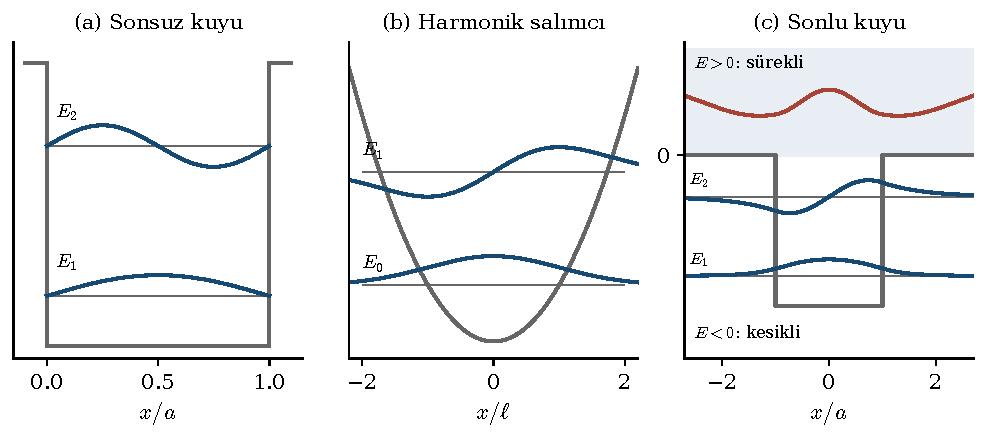
\includegraphics[width=\linewidth]{figurler/05_spektrumlar.pdf}
 \caption[Kesikli ve sürekli enerji spektrumları]{Sonsuz kuyu ve harmonik salınıcıda kesikli spektrum;
 sonlu çekici kuyuda kesikli bağlı durumlarla sürekli saçılma
 spektrumunun birlikte bulunması. Dalga fonksiyonları ilgili enerji
 çizgileri etrafında kaydırılarak gösterilmiştir; dalga genliğinin
 ölçeği enerjiden bağımsızdır.}
 \label{fig:05_spektrumlar}
\end{figure}

\subsubsection{Bir başlangıç durumunun zamanla gelişimi}

Hamiltonyen zamandan bağımsızsa her enerji bileşeni kendi fazıyla
evrilir. Kesikli spektrumda,
\begin{equation}
 \boxed{\Psi(x,t)=\sum_n c_nu_n(x)e^{-iE_nt/\hbar}}
 \label{eq:05_genel_zaman}
\end{equation}
olur. Birden fazla farklı enerji içerildiğinde genel çözüm tek bir
$\psi(x)T(t)$ çarpımı biçiminde ayrılamaz; değişkenlerine ayrılabilenler
tek enerjiye sahip durağan çözümlerdir. Lineerlik sayesinde bunların
toplamı da Schrödinger denkleminin çözümüdür.

Karışık spektrum için benzer biçimde,
\begin{equation}
 \Psi(x,t)=\sum_n c_nu_n(x)e^{-iE_nt/\hbar}
 +\sum_\alpha\int_0^{\infty}
 c_\alpha(E)u_{E\alpha}(x)e^{-iEt/\hbar}\,dE
 \label{eq:05_karisik_zaman}
\end{equation}
yazılır. Buradaki $c_n$ ve $c_\alpha(E)$ katsayıları başlangıç
koşuluyla belirlenir. Zamandan bağımsız Hamiltonyen altında enerji
ölçüm olasılıkları sabittir; buna rağmen farklı enerji bileşenlerinin
göreli fazları değiştiği için konum olasılık yoğunluğu zamanla
değişebilir.

% Kaynak PDF s. 6--16; s. 15--16 alıntı açıklamalarının kavramsal içeriği.
\subsection{Diğer Gözlenebilirler}
\label{sec:05_gozlenebilirler}

Enerji, momentum, konum, açısal momentum, parite ve spin deneysel
olarak ölçülebilen fiziksel niceliklere, yani \emph{gözlenebilirlere}
örnektir. Kuantum mekaniğinde bunlar uygun işlemcilerle temsil edilir.
Bu bölümde enerji dışında önce momentum örneğini inceleyelim.

\subsubsection{Momentum özfonksiyonları ve sürekli spektrum}

Momentumun özdeğer denklemi,
\begin{equation}
 \hat p u_p(x)=-i\hbar\frac{du_p(x)}{dx}=p u_p(x)
\end{equation}
olur. Tam gerçek doğru üzerinde $p$ herhangi bir reel değer alabilir.
Denklemin çözümleri,
\begin{equation}
 \boxed{u_p(x)=\frac{1}{\sqrt{2\pi\hbar}}e^{ipx/\hbar}}
 \label{eq:05_momentum_ozfonksiyon}
\end{equation}
biçimindedir. Bu düzlem dalgalar sıradan anlamda birim norma sahip
değildir; tüm gerçek doğru üzerinde kareleri integrallenemez.
Buradaki katsayı \emph{Dirac-delta normalizasyonu} içindir:
\begin{equation}
 \int_{-\infty}^{\infty}u_p^*(x)u_{p'}(x)\,dx
 =\delta(p-p').
 \label{eq:05_momentum_delta_norm}
\end{equation}
Dolayısıyla sürekli spektrumun özfonksiyonları \emph{genelleştirilmiş
özfonksiyonlar} olarak anlaşılmalıdır. Normalize edilebilir fiziksel
bir dalga paketi ise bunların sürekli toplamıyla kurulur:
\begin{equation}
 \psi(x)=\int_{-\infty}^{\infty}\phi(p)u_p(x)\,dp
 =\frac{1}{\sqrt{2\pi\hbar}}
   \int_{-\infty}^{\infty}\phi(p)e^{ipx/\hbar}\,dp.
 \label{eq:05_momentum_acilim}
\end{equation}
Açılım katsayısı,
\begin{equation}
 \phi(p)=\int_{-\infty}^{\infty}u_p^*(x)\psi(x)\,dx
 =\frac{1}{\sqrt{2\pi\hbar}}
   \int_{-\infty}^{\infty}\psi(x)e^{-ipx/\hbar}\,dx
 \label{eq:05_momentum_katsayi}
\end{equation}
ile bulunur. $\phi(p)$ momentum uzayındaki dalga fonksiyonudur.
Normalize edilmiş bir durumda,
\begin{equation}
 \int|\phi(p)|^2\,dp=1,
 \qquad \operatorname{Prob}(p\le p_{\text{ölçüm}}\le p+dp)
 =|\phi(p)|^2\,dp
\end{equation}
olur; ikinci eşitlik sonsuz küçük aralık için olasılık yoğunluğu
ifadesidir. Sürekli bir dağılımda belirli tek bir momentum değerinin
olasılığı yerine bir momentum aralığının olasılığı konuşulur.

\subsubsection{Genel bir gözlenebilirin özdeğer denklemi}

$\hat A$ ile temsil edilen bir gözlenebilir için,
\begin{equation}
 \hat A u_a(x)=a u_a(x)
 \label{eq:05_genel_ozdeger}
\end{equation}
yazılır. İzinli ölçüm sonuçları $a$ özdeğerleridir. Fiziksel ölçüm
sonuçları reel olduğundan gözlenebilirleri kendine eşlenik
işlemcilerle temsil ederiz. Ders kitabı düzeyindeki kullanımda bu
özellik genellikle \emph{Hermitlik} olarak adlandırılır; işlemcinin
tanım kümesi ve sınır şartlarının da önemli olduğunu aşağıda ve
bölüm sonundaki ekte açıklayacağız.

Yalnızca özdeğerlerin reel olması, tek başına herhangi bir işlemcinin
Hermit olduğunu göstermeye yetmez. Kullanacağımız belirleyici koşul,
bir sonraki alt bölümde verilen iç çarpım eşitliğidir.

Kesikli bir spektrumun ortonormal özfonksiyonları için,
\begin{equation}
 \int u_{a_j}^*(x)u_{a_k}(x)\,dx=\delta_{jk}
\end{equation}
ve sürekli spektrumda,
\begin{equation}
 \int u_a^*(x)u_{a'}(x)\,dx=\delta(a-a')
\end{equation}
geçerlidir. Aynı özdeğere ait birden fazla bağımsız çözüm varsa
özfonksiyonlara ek bir indis eklenir. Şimdilik dejenere olmayan
kesikli durumu kullanarak,
\begin{equation}
 \psi(x)=\sum_j c_j u_{a_j}(x)
 \label{eq:05_a_acilim}
\end{equation}
yazalım. Her iki tarafı $u_{a_k}^*$ ile çarpıp integre etmek,
\begin{align}
 \int u_{a_k}^*(x)\psi(x)\,dx
 &=\sum_j c_j\int u_{a_k}^*(x)u_{a_j}(x)\,dx\\
 &=\sum_j c_j\delta_{kj}=c_k
\end{align}
verir. Dolayısıyla,
\begin{equation}
 \boxed{c_j=\int u_{a_j}^*(x)\psi(x)\,dx}
 \label{eq:05_projeksiyon}
\end{equation}
olur. Sürekli durumda toplam yerine integral geçer:
\begin{equation}
 \psi(x)=\int c(a)u_a(x)\,da,
 \qquad c(a)=\int u_a^*(x)\psi(x)\,dx.
\end{equation}

\subsubsection{Açılım katsayılarının ölçüm yorumu}

Aynı normalize edilmiş $\psi$ durumunda hazırlanmış çok sayıda sistem
üzerinde $A$ ölçümü yapıldığını düşünelim. Kesikli ve dejenere olmayan
spektrumda ölçümün $a_j$ sonucunu verme olasılığı,
\begin{equation}
 P(a_j)=|c_j|^2
 \label{eq:05_born}
\end{equation}
olur. Bütün olası sonuçların olasılıkları toplamı birdir:
\begin{align}
 1=\int|\psi(x)|^2\,dx
 &=\sum_{j,k}c_j^*c_k\int u_{a_j}^*(x)u_{a_k}(x)\,dx\\
 &=\boxed{\sum_j|c_j|^2}.
 \label{eq:05_katsayi_norm}
\end{align}
İdeal bir projektif ölçüm $a_j$ sonucunu verirse, dejenere olmayan
durumda ölçüm sonrası durum bir faz dışında $u_{a_j}$ olur. Araya
zamanla evrim veya başka bir etkileşim girmeden ölçüm hemen
tekrarlanırsa aynı sonuç elde edilir. Dejenerelik varsa ölçüm, durumu
tek bir önceden belirli vektöre değil ilgili özuzaya yansıtır.

Bu olasılık yorumu beklenen değer için de,
\begin{equation}
 \langle A\rangle=\sum_j a_j|c_j|^2
 =\int\psi^*(x)\hat A\psi(x)\,dx
 \label{eq:05_beklenen}
\end{equation}
sonucunu verir. Sürekli spektrumda ise
$\langle A\rangle=\int a|c(a)|^2da$ olur; bu ifadeler ilgili
integral ve toplamlar var olduğunda kullanılır.

\subsubsection{Tamlık bağıntısı}

Denk.~\eqref{eq:05_projeksiyon}'u açılıma yerleştirerek tamlığın
integral biçimini bulalım:
\begin{align}
 \psi(x)&=\sum_j u_{a_j}(x)
                 \int u_{a_j}^*(y)\psi(y)\,dy\\
 &=\int\left[\sum_j u_{a_j}(x)u_{a_j}^*(y)\right]\psi(y)\,dy.
\end{align}
Bu eşitliğin her uygun $\psi$ için geçerli olması,
\begin{equation}
 \boxed{\sum_j u_{a_j}(x)u_{a_j}^*(y)=\delta(x-y)}
 \label{eq:05_tamlik}
\end{equation}
\emph{tamlık bağıntısını} verir. Bu, dağılımlar anlamında bir
eşitliktir: iki tarafın etkisi uygun bir fonksiyonla integre
edildiğinde aynıdır. Sürekli spektrum için,
\begin{equation}
 \int u_a(x)u_a^*(y)\,da=\delta(x-y)
 \label{eq:05_surekli_tamlik}
\end{equation}
yazılır; karışık spektrumda kesikli toplam ve sürekli integral
birlikte bulunur.

Tamlık bağıntısının anlamı, açılımda hiçbir bağımsız bileşenin eksik
kalmamasıdır. Bir ortonormal set eksikse aynı toplam birim işlemciyi
değil, yalnızca o setin gerdiği altuzaya yansıtmayı temsil eder.

Bunu sıradan vektörlerle karşılaştıralım. Üç boyutta ortonormal
$\mathbf e_i$ birim vektörleriyle,
\begin{equation}
 \mathbf v=\sum_{i=1}^3v_i\mathbf e_i,
 \qquad v_i=\mathbf e_i\cdot\mathbf v,
 \qquad |\mathbf v|^2=\sum_i|v_i|^2
\end{equation}
yazılır. Reel baz karmaşık bileşenlerle kullanıldığında son eşitlikte
kompleks eşlenik alınır. Birim uzunlukta bir vektör için
$\sum_i|v_i|^2=1$ olur; bu, dalga fonksiyonu açılımındaki
$\sum_j|c_j|^2=1$ eşitliğinin sonlu boyutlu karşılığıdır.

Dirac gösterimiyle aynı fikir,
\begin{equation}
 \sum_j|u_j\rangle\langle u_j|=\hat I,
 \qquad \langle x|u_j\rangle=u_j(x),
 \qquad\langle x|y\rangle=\delta(x-y)
\end{equation}
olarak yazılır. Sol ve sağdan sırasıyla $\langle x|$ ve
$|y\rangle$ ile çarpmak Denk.~\eqref{eq:05_tamlik}'i verir.

\begin{figure}[hbtp]
 \centering
 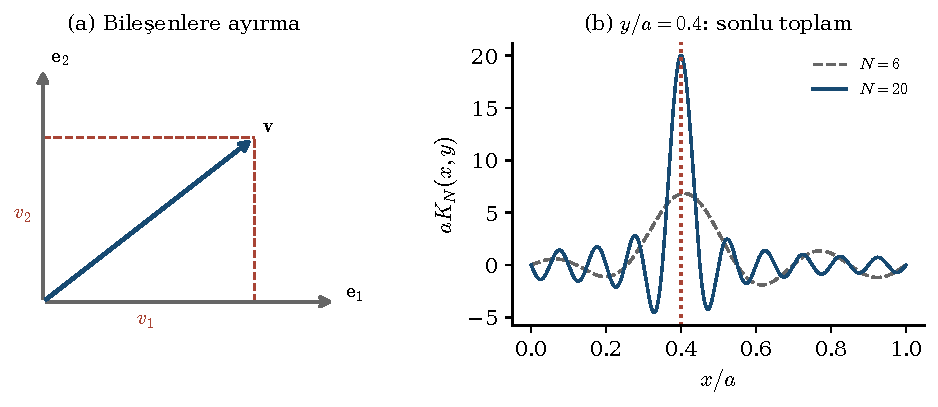
\includegraphics[width=\linewidth]{figurler/05_tamlik.pdf}
 \caption[Tamlık bağıntısı ve vektör benzetimi]{Tamlığın vektör benzetimi ve sonsuz kuyu örneği.
 Solda bir vektörün ortonormal bileşenleri gösterilmiştir. Sağda,
 $K_N(x,y)=\sum_{n=1}^N u_n(x)u_n^*(y)$ sonlu toplamları
 $y/a=0.4$ için çizilmiştir. $N$ arttıkça tepe daralır; delta
 limitinin anlamı noktasal yakınsamadan ziyade uygun fonksiyonlar
 üzerindeki integral etkisidir.}
 \label{fig:05_tamlik}
\end{figure}

\subsubsection{Tamlık bağıntısının iki uygulaması}

\paragraph{Sonsuz kuyunun sinüs bazı.}
$0<x<a$ aralığındaki sonsuz kuyunun normalize edilmiş
özfonksiyonları,
\begin{equation}
 u_n(x)=\sqrt{\frac{2}{a}}\sin\frac{n\pi x}{a},
 \qquad n=1,2,\ldots
\end{equation}
olduğundan tamlık,
\begin{equation}
 \frac{2}{a}\sum_{n=1}^{\infty}
 \sin\frac{n\pi x}{a}\sin\frac{n\pi y}{a}
 =\delta(x-y),\qquad 0<x,y<a
 \label{eq:05_sinus_tamlik}
\end{equation}
biçimini alır. Bu fonksiyonlar $0<x<a$ aralığının tam sinüs bazıdır;
merkezi orijin olan bir kuyunun yalnızca tek pariteli özfonksiyonları
olarak alınırsa tüm Hilbert uzayını kapsamazlar.

$X=x/a$, $Y=y/a$ ve $a>0$ için
$\delta(X-Y)=a\delta(x-y)$ olduğundan,
\begin{equation}
 2\sum_{n=1}^{\infty}\sin(n\pi X)\sin(n\pi Y)
 =\delta(X-Y),\qquad 0<X,Y<1
 \label{eq:05_sinus_boyutsuz}
\end{equation}
elde edilir. Toplam indisini negatif tamsayılara genişletebiliriz:
$\sin(-n\pi X)\sin(-n\pi Y)=\sin(n\pi X)\sin(n\pi Y)$ ve $n=0$
terimi sıfır olduğundan,
\begin{equation}
 \sum_{n=-\infty}^{\infty}\sin(n\pi X)\sin(n\pi Y)
 =\delta(X-Y),\qquad 0<X,Y<1
\end{equation}
olur. Eşitliğin belirtilen aralığa ait olduğu unutulmamalıdır;
tüm gerçek doğruya periyodik uzatıldığında ek görüntü terimleri
ortaya çıkar.

\paragraph{Düzlem dalgalar ve delta dağılımının Fourier gösterimi.}
Momentum bazının tamlık bağıntısı,
\begin{align}
 \delta(x-y)&=\int_{-\infty}^{\infty}u_p(x)u_p^*(y)\,dp\\
 &=\frac{1}{2\pi\hbar}\int_{-\infty}^{\infty}
 e^{ip(x-y)/\hbar}\,dp
\end{align}
olur. $p=\hbar k$ dönüşümünden,
\begin{equation}
 \boxed{\delta(x-y)=\frac{1}{2\pi}
       \int_{-\infty}^{\infty}e^{ik(x-y)}\,dk}
 \label{eq:05_delta_fourier}
\end{equation}
bulunur. İntegral sıradan yakınsak bir integral olarak değil,
dağılım anlamında okunur. Örneğin bir Gauss düzenleyicisiyle,
\begin{equation}
 \frac{1}{2\pi}\int e^{-\epsilon k^2}e^{ik(x-y)}\,dk
 =\frac{1}{\sqrt{4\pi\epsilon}}
       e^{-(x-y)^2/(4\epsilon)}
 \xrightarrow[\epsilon\to0^+]{}\delta(x-y)
\end{equation}
yazılması bu anlamı görünür kılar.

% Kaynak PDF s. 17--22.
\subsection{Vektör Uzayları ve İşlemciler}
\label{sec:05_vektor_uzayi}

Özfonksiyon açılımları ile sıradan vektörlerin baz vektörleri
cinsinden yazılması arasındaki benzetim yalnızca biçimsel değildir.
Dalga fonksiyonları bir karmaşık vektör uzayında ele alınabilir.
Örneğin $\psi_A$ ve $\psi_B$ iki kare integrallenebilir fonksiyonsa,
\begin{equation}
 \psi_C=\alpha\psi_A+\beta\psi_B
\end{equation}
de aynı uzayın bir elemanıdır. Bunun bir fiziksel durum dalga
fonksiyonu olarak kullanılması için sıfırdan farklı olması ve uygun
şekilde normalize edilmesi gerekir. Zamana bağlı Schrödinger
denkleminin çözümlerinin doğrusal birleşimi de aynı Hamiltonyen için
bir çözümdür.

Vektörlerin skaler çarpımının fonksiyon uzayındaki karşılığı,
\begin{equation}
 \langle\phi|\psi\rangle
 =\int\phi^*(x)\psi(x)\,dx
 \label{eq:05_ic_carpim}
\end{equation}
iç çarpımıdır. Bu tanım birinci girdide eşlenik doğrusal, ikinci
girdide doğrusaldır ve,
\begin{equation}
 \langle\phi|\psi\rangle^*=\langle\psi|\phi\rangle,
 \qquad \|\psi\|^2=\langle\psi|\psi\rangle\ge0
\end{equation}
özelliklerini taşır. Bu iç çarpımla tamamlanmış uzay
\emph{Hilbert uzayı} olarak adlandırılır. Konum gösterimindeki
spin içermeyen tek parçacık problemi için kullanılan uzay genellikle
$L^2(\mathbb R)$'dir. Sonsuz boyutlu olması yalnızca sürekli spektruma
bağlı değildir: sonsuz kuyu gibi kesikli bir baz da sonsuz sayıda
bağımsız fonksiyon içerebilir.

\subsubsection{Doğrusal işlemciler}

Bir işlemci, tanım kümesindeki bir vektörü başka bir vektöre götürür.
Doğrusal bir $\hat A$ işlemcisi için,
\begin{equation}
 \boxed{\hat A(\alpha\psi_1+\beta\psi_2)
 =\alpha\hat A\psi_1+\beta\hat A\psi_2}
 \label{eq:05_dogrusal}
\end{equation}
geçerlidir. $\alpha$ ve $\beta$ karmaşık sayılardır.
Örneğin türev alma ve belirli bir fonksiyonla çarpma doğrusaldır.
İşlemcilerin çarpımında sıra önemlidir: $\hat A\hat B\psi$ yazımı,
önce $\hat B$'nin sonra $\hat A$'nın etki ettiğini gösterir.

\subsubsection{Hermit eşlenik ve Hermitlik}

$\hat Q$ işlemcisinin \emph{Hermit eşleniği}, uygun $\phi$ ve $\psi$
için,
\begin{equation}
 \boxed{\langle\phi|\hat Q^\dagger\psi\rangle
       =\langle\hat Q\phi|\psi\rangle}
 \label{eq:05_eslenik_tanim}
\end{equation}
ile tanımlanır. İntegral gösteriminde,
\begin{equation}
 \int\phi^*(x)\hat Q^\dagger\psi(x)\,dx
 =\int[\hat Q\phi(x)]^*\psi(x)\,dx
\end{equation}
olur. Buradaki eşlenik alma, yalnızca katsayıların kompleks
eşleniğini almak değildir; türevler ve sınır terimleri de hesaba
katılır. Matris gösteriminde ise,
\begin{equation}
 Q^\dagger=(Q^*)^{\mathsf T},
 \qquad (Q^\dagger)_{jk}=Q_{kj}^*
\end{equation}
kompleks eşlenik transpozdur.

Normalize edilmiş bir $\psi$ için,
\begin{align}
 \langle Q\rangle^*
 &=\left[\int\psi^*\hat Q\psi\,dx\right]^*\\
 &=\int(\hat Q\psi)^*\psi\,dx
 =\int\psi^*\hat Q^\dagger\psi\,dx
 =\langle Q^\dagger\rangle
 \label{eq:05_beklenen_eslenik}
\end{align}
elde edilir. Hermit bir işlemci,
\begin{equation}
 \boxed{\hat A=\hat A^\dagger}
 \label{eq:05_hermit}
\end{equation}
koşulunu sağlar; dolayısıyla beklenen değerleri reeldir:
\begin{equation}
 \langle A\rangle^*=\langle A\rangle.
\end{equation}
Bu reel olma koşulu tek bir seçilmiş durumda değil, işlemcinin
uygun tanım kümesindeki bütün durumlarda sağlanmalıdır.

\begin{tcolorbox}
Diferansiyel işlemcilerde $\hat A=\hat A^\dagger$ eşitliği,
matematiksel olarak işlemcilerin tanım kümelerinin de aynı olmasını
gerektirir. Yalnızca
$\langle\phi|\hat A\psi\rangle=\langle\hat A\phi|\psi\rangle$
integral koşulu işlemcinin kendi tanım kümesinde \emph{simetrik}
olduğunu gösterir. Kendine eşleniklik bunun daha güçlü biçimidir.
Bu bölümdeki Hermit işlemci ifadeleri uygun sınır şartlarıyla birlikte
kullanılacaktır. Momentum örneği bölüm sonundaki ekte ele alınmıştır.
\end{tcolorbox}

\subsubsection{Reel özdeğerler ve dik özfonksiyonlar}

$\hat A u_a=a u_a$ olsun. $u_a$ normalize edilmişse,
\begin{equation}
 \langle u_a|\hat A u_a\rangle=a,
 \qquad\langle\hat A u_a|u_a\rangle=a^*.
\end{equation}
Hermitlik iki iç çarpımı eşitlediği için $a=a^*$, yani özdeğer
reeldir. Genelleştirilmiş sürekli özfonksiyonlar için aynı sonuç
spektral açılımın uygun anlamında geçerlidir.

İki özfonksiyon için,
\begin{equation}
 \hat A u_1=a_1u_1,\qquad\hat A u_2=a_2u_2
\end{equation}
yazalım. Hermitlik kullanıldığında,
\begin{align}
 a_2\langle u_1|u_2\rangle
 &=\langle u_1|\hat A u_2\rangle
 =\langle\hat A u_1|u_2\rangle\\
 &=a_1\langle u_1|u_2\rangle
\end{align}
olduğundan,
\begin{equation}
 (a_2-a_1)\langle u_1|u_2\rangle=0
\end{equation}
bulunur. Böylece farklı özdeğerlere karşılık gelen özfonksiyonların
dikliği genel olarak gösterilmiş olur.

\subsubsection{Çarpımın Hermit eşleniği}

İki işlemcinin çarpımında Hermit eşlenik alınırken sıra tersine döner.
Bunu iç çarpımdan adım adım görelim:
\begin{align}
 \langle\hat A\hat B\phi|\psi\rangle
 &=\langle\hat B\phi|\hat A^\dagger\psi\rangle\\
 &=\langle\phi|\hat B^\dagger\hat A^\dagger\psi\rangle.
\end{align}
Dolayısıyla uygun ortak tanım kümesinde,
\begin{equation}
 \boxed{(\hat A\hat B)^\dagger
             =\hat B^\dagger\hat A^\dagger}
 \label{eq:05_carpim_eslenik}
\end{equation}
yazılır. Sonlu boyutlu matrislerde bu eşitlik koşulsuz geçerlidir;
sınırsız diferansiyel işlemcilerde çarpımların tanımlı olduğu kümeler
de denetlenmelidir. Aynı kural daha uzun çarpımlara genişler:
\begin{equation}
 (\hat A\hat B\hat C\cdots\hat Z)^\dagger
 =\hat Z^\dagger\cdots\hat C^\dagger\hat B^\dagger\hat A^\dagger.
\end{equation}
Ayrıca,
\begin{equation}
 (\alpha\hat A+\beta\hat B)^\dagger
 =\alpha^*\hat A^\dagger+\beta^*\hat B^\dagger
\end{equation}
olur. Bu kurallarla,
\begin{equation}
 \hat Q+\hat Q^\dagger,\qquad
 i(\hat Q-\hat Q^\dagger),\qquad
 \hat Q\hat Q^\dagger
\end{equation}
ifadelerinin formal olarak Hermit olduğu görülebilir. Örneğin,
\begin{equation}
 [i(\hat Q-\hat Q^\dagger)]^\dagger
 =-i(\hat Q^\dagger-\hat Q)
 =i(\hat Q-\hat Q^\dagger).
\end{equation}
Sınırsız işlemcilerde bunların kendine eşlenik gerçekleşimleri için
tanım kümesi koşulları yine ayrıca önemlidir.

İki Hermit işlemcinin çarpımı ise her zaman Hermit değildir:
\begin{equation}
 (\hat A\hat B)^\dagger=\hat B\hat A.
\end{equation}
Bu çarpımın Hermit olması için, aynı uygun uzayda,
$\hat A\hat B=\hat B\hat A$ olması gerekir. İşlemci sırasının
etkisini ölçen,
\begin{equation}
 \boxed{[\hat A,\hat B]\equiv\hat A\hat B-\hat B\hat A}
 \label{eq:05_komutator_tanim}
\end{equation}
ifadesine \emph{komütatör} denir. $[\hat A,\hat B]=0$ olduğunda
$\hat A$ ve $\hat B$ \emph{komüte eder} deriz.

% Kaynak PDF s. 23--33; s. 27, 31--32'deki serbest parçacık türetmeleri
% konu sırasına göre bir araya getirilmiştir.
\subsection{Dejenerelik (Yozlaşma) ve Eşzamanlı Gözlenebilirler}
\label{sec:05_dejenerelik}

İki gözlenebilirin ortak özfonksiyonlara sahip olması, bu niceliklerin
aynı durumda belirli değerler taşıyabilmesini sağlar. Ancak ortak
birkaç özfonksiyonun bulunması ile bütün uzayı kapsayan ortak bir
özfonksiyon bazının bulunmasını ayırmak gerekir.

\subsubsection{Ortak özfonksiyonlar ve komütasyon}

Bir $u_{ab}$ fonksiyonu hem $\hat A$'nın hem $\hat B$'nin
özfonksiyonu olsun:
\begin{equation}
 \hat A u_{ab}=a u_{ab},\qquad
 \hat B u_{ab}=b u_{ab}.
\end{equation}
Bu durumda,
\begin{align}
 \hat A\hat B u_{ab}&=\hat A(bu_{ab})=ab u_{ab},\\
 \hat B\hat A u_{ab}&=\hat B(au_{ab})=ab u_{ab}
\end{align}
olduğundan $[\hat A,\hat B]u_{ab}=0$ bulunur. Yalnızca tek bir
fonksiyonda bu sonucun bulunması, komütatörün işlemci olarak sıfır
olduğunu kanıtlamaz.

Buna karşılık $u_{ab}$'ler tam bir ortak bazsa,
\begin{equation}
 \psi=\sum_{a,b}c_{ab}u_{ab}
\end{equation}
açılımı kullanılarak,
\begin{equation}
 [\hat A,\hat B]\psi
 =\sum_{a,b}c_{ab}[\hat A,\hat B]u_{ab}=0
\end{equation}
elde edilir. Böylece ortak tam baz komütasyona götürür. Sürekli
spektrumda ilgili toplamlar integrallerle tamamlanır.

Ters yönden, $[\hat A,\hat B]=0$ ve $\hat A u_a=a u_a$ ise,
\begin{equation}
 \hat A(\hat B u_a)=\hat B\hat A u_a=a(\hat B u_a)
 \label{eq:05_ozuzay_korunur}
\end{equation}
olur. Yani $\hat B u_a$ sıfır değilse aynı $a$ özuzayında kalır.
$a$ dejenere değilse bu özuzay tek boyutludur ve
$\hat B u_a=b u_a$ sonucu çıkar. Böylece $u_a$ ortak özfonksiyondur.

Aynı özdeğere karşılık birden fazla doğrusal bağımsız özfonksiyon
varsa bu duruma \emph{dejenerelik} denir. Örneğin,
\begin{equation}
 \hat A u_a^{(1)}=a u_a^{(1)},\qquad
 \hat A u_a^{(2)}=a u_a^{(2)}
\end{equation}
ike bağımsız çözüm varsa $a$ iki kat dejenere bir özdeğerdir.
Dejenerelik komütasyonun bozulduğu anlamına gelmez. Komüte eden
$\hat B$, bu iki fonksiyonu aynı özuzay içinde birbirine
karıştırabilir:
\begin{equation}
 \hat B u_a^{(j)}=\sum_k B_{kj}^{(a)}u_a^{(k)}.
\end{equation}
Bu özuzay içindeki Hermit $B^{(a)}$ matrisini köşegenleştirmek,
$\hat A$ ve $\hat B$ için ortak özfonksiyonları verir. Dolayısıyla
başlangıçta seçilen dejenere bazın her elemanının ortak özfonksiyon
olması gerekmez; uygun doğrusal birleşimler seçilebilir.

Bu ortak baz anlatımı sonlu boyutta ve burada kullanılan standart
kesikli spektrum örneklerinde doğrudan uygulanır. Genel sınırsız
kendine eşlenik işlemciler için eşzamanlı spektral ayrışım, yalnızca
formal bir komütatör hesabından daha güçlü koşullar gerektirir.

\subsubsection{Serbest parçacık: enerji, parite ve momentum}

Serbest parçacıkta,
\begin{equation}
 \hat H=-\frac{\hbar^2}{2m}\frac{d^2}{dx^2}
       =\frac{\hat p^2}{2m}
\end{equation}
olduğundan $\hat H$ ile $\hat p$ komüte eder. $k>0$ için,
\begin{equation}
 c(x)=\cos kx,\qquad s(x)=\sin kx
\end{equation}
fonksiyonları aynı $E=\hbar^2k^2/(2m)$ enerji özdeğerine sahiptir:
\begin{equation}
 \hat Hc=Ec,\qquad \hat Hs=Es.
\end{equation}
Tam doğru üzerinde bunlar genelleştirilmiş özfonksiyonlardır;
burada ortak enerji altuzayındaki yapıyı göstermek için sabit
çarpanlarını yazmıyoruz.

Parite işlemcisini momentum işlemcisinden ayırmak için $\hat\Pi$
ile gösterelim:
\begin{equation}
 (\hat\Pi\psi)(x)=\psi(-x).
\end{equation}
Bu durumda,
\begin{equation}
 \hat\Pi c=+c,\qquad\hat\Pi s=-s.
\end{equation}
Dolayısıyla $c$ ve $s$, enerjinin ve paritenin ortak
özfonksiyonlarıdır. Momentumun etkisi ise,
\begin{equation}
 \hat p c=i\hbar k\,s,
 \qquad \hat p s=-i\hbar k\,c
 \label{eq:05_p_sin_cos}
\end{equation}
şeklindedir. Görüldüğü gibi $c$ ve $s$ tek tek momentum
özfonksiyonları değildir; momentum aynı enerjiye ait iki çözümü
birbirine dönüştürür.

Bununla birlikte komütatörü bu bazda da hesaplayabiliriz:
\begin{align}
 [\hat H,\hat p]c
 &=\hat H(i\hbar k s)-\hat p(Ec)
 =i\hbar k E s-E i\hbar k s=0,\\
 [\hat H,\hat p]s&=0.
\end{align}
Yani komütatörün sıfır olması, hesapta kullanılan fonksiyonun her
iki işlemcinin de özfonksiyonu olmasını gerektirmez.

Ortak özfonksiyonları bulmak için $c$ ve $s$'nin doğrusal
birleşimlerini alalım:
\begin{equation}
 v_+(x)=c(x)+i s(x)=e^{ikx},\qquad
 v_-(x)=c(x)-i s(x)=e^{-ikx}.
\end{equation}
Bunlara işlemciler etki ettirildiğinde,
\begin{align}
 \hat H v_\pm&=\frac{\hbar^2k^2}{2m}v_\pm=E v_\pm,\\
 \hat p v_\pm&=\pm\hbar k v_\pm
 \label{eq:05_ortak_hp}
\end{align}
elde edilir. Enerji özdeğeri iki kat dejenereyken bu iki durumda
momentum özdeğerleri farklıdır. Enerjinin yanına momentumun işaretini
belirtmek, bu dejenereliği ayırır.

Aynı hesap $\{c,s\}$ bazında bir $2\times2$ matris olarak da yazılır:
\begin{equation}
 H=E\begin{pmatrix}1&0\\0&1\end{pmatrix},\qquad
 p=\hbar k\begin{pmatrix}0&-i\\i&0\end{pmatrix},\qquad
 \Pi=\begin{pmatrix}1&0\\0&-1\end{pmatrix}.
 \label{eq:05_serbest_matrisler}
\end{equation}
Momentum matrisinin özvektörleri $(1,\pm i)^{\mathsf T}/\sqrt2$
olup yukarıdaki doğrusal birleşimleri verir.

\begin{figure}[hbtp]
 \centering
 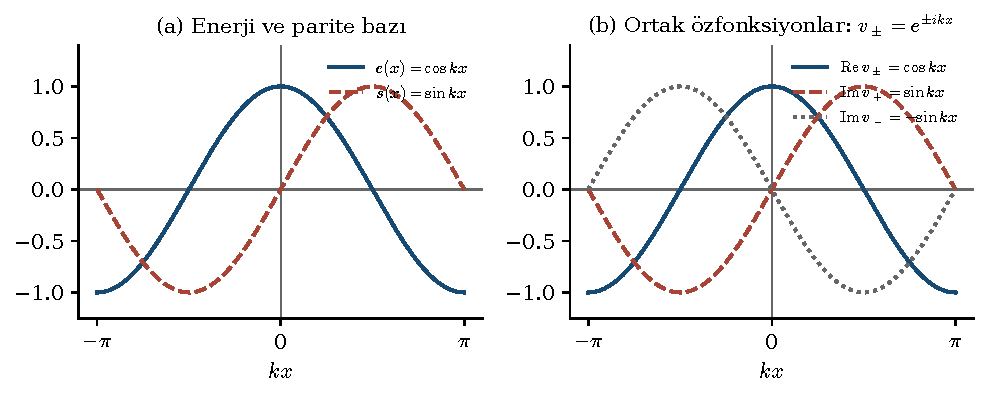
\includegraphics[width=\linewidth]{figurler/05_dejenere_bazlar.pdf}
 \caption[Serbest parçacıkta dejenere bazlar]{Serbest parçacığın aynı enerjiye ait iki farklı baz seçimi.
 Sinüs ve kosinüs enerji ile paritenin ortak özfonksiyonlarıdır.
 Bunların $c\pm is$ birleşimleri enerji ile momentumun ortak
 özfonksiyonlarını verir. Sağ panel karmaşık fonksiyonların reel ve
 sanal kısımlarını gösterir.}
 \label{fig:05_dejenere_bazlar}
\end{figure}

Parite ile momentum ise komüte etmez. Çünkü,
\begin{equation}
 \hat\Pi\hat p\psi=-\hat p\hat\Pi\psi,
 \qquad [\hat\Pi,\hat p]=-2\hat p\hat\Pi.
\end{equation}
Örneğin çift $c$ fonksiyonunda,
\begin{equation}
 [\hat\Pi,\hat p]c
 =-i\hbar k s-i\hbar k s=-2i\hbar k s\ne0.
\end{equation}
Böylece,
\begin{equation}
 [\hat H,\hat p]=0,\qquad [\hat H,\hat\Pi]=0,
 \qquad [\hat\Pi,\hat p]\ne0
 \label{eq:05_komutasyon_ornek}
\end{equation}
olabilir. Komütasyon geçişli bir ilişki değildir: iki işlemcinin
ayrı ayrı aynı Hamiltonyenle komüte etmesi, birbirleriyle komüte
etmelerini gerektirmez.

\subsubsection{Birbiriyle komüte eden gözlenebilirlerin tam seti}

Bir gözlenebilirin özdeğeri durumu tek başına ayırt etmiyorsa,
onunla komüte eden başka gözlenebilirlerin özdeğerleri de
belirtilebilir. Uygun ortak özfonksiyonları,
\begin{equation}
 u_{a,b,\ldots,z}
\end{equation}
ile gösterebiliriz. Özdeğerler bir durum vektörünü genel faz dışında
tek olarak belirliyorsa, kullanılan gözlenebilirler
\emph{birbiriyle komüte eden gözlenebilirlerin tam seti}ni oluşturur.

Burada dejenereliğin ortak özdeğer etiketleriyle giderilmesi,
enerji seviyesinin fiziksel olarak yarılması anlamına gelmez.
Serbest parçacık örneğinde iki durum aynı enerjiye sahip olmaya
devam eder; yalnızca momentumlarıyla ayırt edilirler. Bütün
nicelikleri aynı anda kesin belirlemek ise genel olarak mümkün
değildir. Bunun sınırını komütatörler ve belirsizlik bağıntıları
belirler.

\subsubsection{Komütatör ve belirsizlik bağıntısı}

Normalize edilmiş bir durumda iki Hermit gözlenebilirin sapma
kareleri,
\begin{equation}
 (\Delta A)^2=\langle(\hat A-\langle A\rangle)^2\rangle
 =\langle A^2\rangle-\langle A\rangle^2
\end{equation}
ve benzer biçimde $(\Delta B)^2$ ile tanımlanır.
$\delta\hat A=\hat A-\langle A\rangle$ ve
$\delta\hat B=\hat B-\langle B\rangle$ yazalım. Cauchy--Schwarz
 eşitsizliğinden,
\begin{equation}
 (\Delta A)^2(\Delta B)^2
 \ge\left|\langle\delta\hat A\,\delta\hat B\rangle\right|^2
 \ge\left|\operatorname{Im}
           \langle\delta\hat A\,\delta\hat B\rangle\right|^2
\end{equation}
olur. Hermitlik kullanıldığında,
\begin{equation}
 \operatorname{Im}\langle\delta\hat A\,\delta\hat B\rangle
 =\frac{1}{2i}\langle[\hat A,\hat B]\rangle
\end{equation}
bulunduğundan,
\begin{equation}
 \boxed{\Delta A\,\Delta B
 \ge\frac12\left|\langle[\hat A,\hat B]\rangle\right|}
 \label{eq:05_robertson}
\end{equation}
elde edilir. Eşdeğer olarak,
$(\Delta A)^2(\Delta B)^2\ge\frac14\langle i[\hat A,\hat B]\rangle^2$
yazılabilir; $i[\hat A,\hat B]$ Hermit olduğundan bu beklenen değer
reeldir.

Konum ve momentum için komütatörü herhangi bir uygun $f(x)$
fonksiyonuna etki ettirerek hesaplayalım:
\begin{align}
 [\hat p,\hat x]f(x)
 &=-i\hbar\frac{d}{dx}[xf(x)]
   +i\hbar x\frac{df}{dx}\\
 &=-i\hbar f(x).
\end{align}
Böylece,
\begin{equation}
 [\hat p,\hat x]=-i\hbar\hat I,
 \qquad [\hat x,\hat p]=i\hbar\hat I
 \label{eq:05_xp}
\end{equation}
ve,
\begin{equation}
 \boxed{\Delta x\,\Delta p\ge\frac{\hbar}{2}}
\end{equation}
bulunur. Bu hesapta düzlem dalga seçmek gerekmez; düzlem dalganın
kendisi normalize edilemediğinden onun konum varyansını sonluymuş
gibi kullanmak da doğru olmaz. Belirsizlik bağıntısı ilgili
momentleri sonlu olan fiziksel durumlar için uygulanır.

% Kaynak PDF s. 34--40.
\subsection{Zamana Bağlılık ve Klasik Limit}
\label{sec:05_zaman_klasik}

Kuantum teorisinin klasik limitini anlayabilmek için gözlenebilirlerin
beklenen değerlerinin zamanla nasıl değiştiğini incelemeliyiz.
İşlemcinin kendisi zamana açıkça bağlı olabilir; ayrıca durum dalga
fonksiyonu da zamanla gelişir. Bu iki katkı birbirinden ayrılmalıdır.

\subsubsection{Beklenen değerin zaman türevi}

Normalize edilmiş $\Psi(x,t)$ durumunda,
\begin{equation}
 \langle A\rangle(t)=\int\Psi^*(x,t)\hat A(t)\Psi(x,t)\,dx
\end{equation}
yazalım. İntegral ile türevin yer değiştirebildiği uygun
koşullarda çarpımın türevi,
\begin{align}
 \frac{d\langle A\rangle}{dt}
 &=\int\frac{\partial\Psi^*}{\partial t}\hat A\Psi\,dx
 +\int\Psi^*\frac{\partial\hat A}{\partial t}\Psi\,dx
 +\int\Psi^*\hat A\frac{\partial\Psi}{\partial t}\,dx
 \label{eq:05_zaman_uc_terim}
\end{align}
olur. Schrödinger denkleminden,
\begin{equation}
 \frac{\partial\Psi}{\partial t}=\frac{1}{i\hbar}\hat H\Psi
\end{equation}
ve bunun karmaşık eşleniğinden yararlanırsak,
\begin{align}
 \frac{d\langle A\rangle}{dt}
 &=-\frac{1}{i\hbar}\int(\hat H\Psi)^*\hat A\Psi\,dx
 +\left\langle\frac{\partial\hat A}{\partial t}\right\rangle
 +\frac{1}{i\hbar}\int\Psi^*\hat A\hat H\Psi\,dx\\
 &=\left\langle\frac{\partial\hat A}{\partial t}\right\rangle
 +\frac{1}{i\hbar}\int\Psi^*
       (\hat A\hat H-\hat H\hat A)\Psi\,dx
\end{align}
bulunur. İkinci satırda Hamiltonyenin Hermitliğini kullandık.
Sonuç,
\begin{equation}
 \boxed{\frac{d\langle A\rangle}{dt}
 =\left\langle\frac{\partial\hat A}{\partial t}\right\rangle
 +\frac{i}{\hbar}\langle[\hat H,\hat A]\rangle}
 \label{eq:05_genel_ehrenfest}
\end{equation}
veya eşdeğer olarak
$d\langle A\rangle/dt=\langle\partial_t\hat A\rangle
+\langle[\hat A,\hat H]\rangle/(i\hbar)$ şeklindedir.

\subsubsection{Hareket sabitleri}

$\hat A$ zamana açıkça bağlı değilse,
\begin{equation}
 \frac{d\langle A\rangle}{dt}
 =\frac{i}{\hbar}\langle[\hat H,\hat A]\rangle
\end{equation}
olur. Buna ek olarak $[\hat H,\hat A]=0$ ise beklenen değer her
uygun durumda sabittir. Böyle bir gözlenebilire \emph{hareket sabiti}
denebilir. Hamiltonyen zamandan bağımsızsa enerji korunur; ayrıca
Hamiltonyenle komüte eden zamandan bağımsız diğer gözlenebilirler
de korunur.

Burada iki durumu ayırmak gerekir: bir komütatörün belirli bir
durumdaki beklenen değerinin sıfır olması, komütatörün işlemci olarak
sıfır olması demek değildir. Örneğin bir enerji özdurumunda pek çok
beklenen değer sabittir; bu, bütün ilgili işlemcilerin Hamiltonyenle
komüte ettiğini göstermez.

\subsubsection{Konumun beklenen değeri}

$\hat H=\hat p^2/(2m)+V(\hat x)$ olsun. Konum işlemcisinin zamana
açık bağımlılığı yoktur. $V(\hat x)$ ile $\hat x$ komüte eder:
\begin{equation}
 [V(\hat x),\hat x]=0.
\end{equation}
Dolayısıyla,
\begin{equation}
 [\hat H,\hat x]=\frac{1}{2m}[\hat p^2,\hat x].
\end{equation}
Çarpım kuralı,
\begin{equation}
 [\hat A\hat B,\hat C]
 =\hat A[\hat B,\hat C]+[\hat A,\hat C]\hat B
\end{equation}
ile Denk.~\eqref{eq:05_xp} birlikte kullanılırsa,
\begin{align}
 [\hat p^2,\hat x]
 &=\hat p[\hat p,\hat x]+[\hat p,\hat x]\hat p\\
 &=-i\hbar\hat p-i\hbar\hat p=-2i\hbar\hat p
\end{align}
olur. Beklenen değer denklemine yerleştirirsek,
\begin{equation}
 \boxed{\frac{d\langle x\rangle}{dt}
       =\frac{\langle p\rangle}{m}}
 \label{eq:05_ehrenfest_x}
\end{equation}
bulunur. Konumun ortalamasının değişim hızı, momentum ortalamasının
kütleye oranıdır. Konum genel olarak bir hareket sabiti değildir.

\subsubsection{Momentumun beklenen değeri}

Momentumun da zamana açık bağımlılığı bulunmadığından,
\begin{equation}
 \frac{d\langle p\rangle}{dt}
 =\frac{i}{\hbar}\langle[\hat H,\hat p]\rangle
 =\frac{i}{\hbar}\langle[V(\hat x),\hat p]\rangle
\end{equation}
olur; burada $[\hat p^2,\hat p]=0$ kullandık. Potansiyelin yeterince
düzgün olduğu bölgede, uygun bir $f(x)$ için,
\begin{align}
 [V,\hat p]f
 &=V(-i\hbar f')+i\hbar\frac{d}{dx}(Vf)\\
 &=i\hbar V'f.
\end{align}
Böylece,
\begin{equation}
 [V,\hat p]=i\hbar\frac{dV}{dx}
\end{equation}
ve,
\begin{equation}
 \boxed{\frac{d\langle p\rangle}{dt}
       =-\left\langle\frac{dV}{dx}\right\rangle
       =\langle F(x)\rangle}
 \label{eq:05_ehrenfest_p}
\end{equation}
elde edilir. Momentum genel bir potansiyelde korunmaz. Serbest
parçacıkta veya sabit potansiyelde $V'=0$ olduğu için korunur.
Belirli bir durumda ortalama kuvvet sıfırsa o durumda momentum
ortalamasının türevi sıfır olabilir; bu da tek başına her durumda
korunum demek değildir.

Denk.~\eqref{eq:05_ehrenfest_x}'in zaman türevi alınarak iki sonuç
birleştirilebilir:
\begin{equation}
 \boxed{m\frac{d^2\langle x\rangle}{dt^2}
       =-\left\langle\frac{dV}{dx}\right\rangle
       =\langle F(x)\rangle.}
 \label{eq:05_ehrenfest_newton}
\end{equation}
Bu eşitlikler \emph{Ehrenfest teoremi}nin konum ve momentum için
biçimleridir.

\subsubsection{Ortalama kuvvet ile ortalama konumdaki kuvvet}

Klasik bir parçacığın hareketi,
\begin{equation}
 m\frac{d^2x_{\rm kl}}{dt^2}=F(x_{\rm kl})
\end{equation}
ile belirlenir. Kuantum denkleminde ise genel olarak,
\begin{equation}
 \langle F(x)\rangle\ne F(\langle x\rangle)
 \label{eq:05_kuvvet_farki}
\end{equation}
olur. Dolayısıyla $x_{\rm kl}=\langle x\rangle$ özdeşleştirmesi
her potansiyelde otomatik olarak klasik hareket denklemini vermez.

Bu farkı görmek için $X=\langle x\rangle$ etrafında kuvveti Taylor
serisine açalım:
\begin{equation}
 F(x)=F(X)+F'(X)(x-X)+\frac12F''(X)(x-X)^2+\cdots.
\end{equation}
Beklenen değer alındığında $\langle x-X\rangle=0$ ve
$\langle(x-X)^2\rangle=(\Delta x)^2$ olduğundan,
\begin{equation}
 \langle F(x)\rangle
 =F(X)+\frac12F''(X)(\Delta x)^2
   +\frac16F'''(X)\langle(x-X)^3\rangle+\cdots
 \label{eq:05_kuvvet_taylor}
\end{equation}
elde edilir. Dağılım, kuvvetin belirgin değiştiği uzunluk ölçeğine
göre dar kalıyorsa üst mertebe terimler küçüktür ve,
\begin{equation}
 \langle F(x)\rangle\simeq F(\langle x\rangle)
\end{equation}
yaklaşımı yapılabilir. Gerekli koşul yalnızca potansiyelin yavaş
değişmesi değil, dalga paketinin genişliği boyunca kuvvetin yeterince
az eğrilik göstermesidir. Paket zamanla genişlerse bu yaklaşımın
geçerliliği de zaman içinde değişebilir.

Bir örnek olarak yerel bir $V(x)=\beta x^3$ potansiyelinde,
\begin{equation}
 F(x)=-3\beta x^2,\qquad
 \langle F(x)\rangle=-3\beta[X^2+(\Delta x)^2],\qquad
 F(X)=-3\beta X^2
\end{equation}
olur. Aynı merkez konuma sahip iki dağılımın genişlikleri farklıysa
ortalama kuvvetleri de farklı olabilir. Bu örnek yalnızca kuvvet
ortalaması farkını göstermek içindir; kübik potansiyelin tüm uzayda
bağlı durum oluşturduğu varsayılmamaktadır.

\begin{figure}[hbtp]
 \centering
 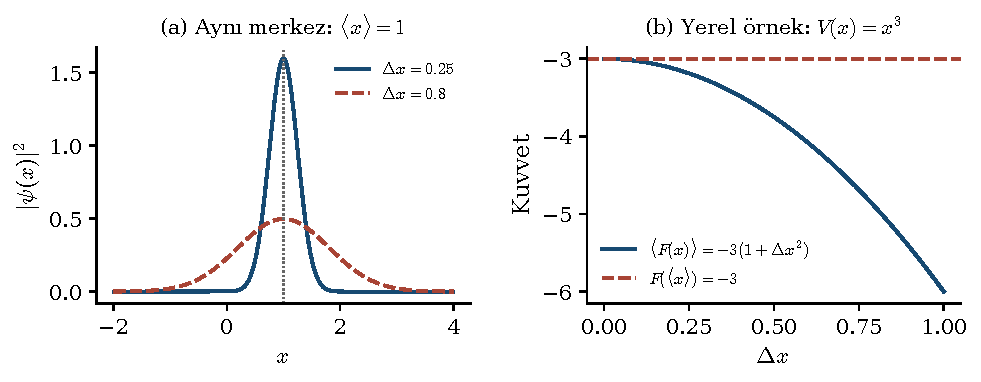
\includegraphics[width=\linewidth]{figurler/05_ehrenfest_kuvvet.pdf}
 \caption[Ortalama kuvvet ile ortalama konumdaki kuvvet]{Aynı ortalama konum, genel olarak aynı ortalama kuvveti
 vermez. Solda merkezleri aynı, genişlikleri farklı iki Gauss
 yoğunluğu gösterilmiştir. Sağda keyfi birimlerle yerel $V=x^3$
 örneğinde $\langle F(x)\rangle$ ile $F(\langle x\rangle)$
 karşılaştırılmıştır.}
 \label{fig:05_ehrenfest_kuvvet}
\end{figure}

Öte yandan sabit veya doğrusal kuvvetlerde $F''=0$ olduğundan,
$\langle F(x)\rangle=F(\langle x\rangle)$ eşitliği dağılımın
genişliğinden bağımsız olarak tamdır. Örneğin harmonik salınıcıda,
\begin{equation}
 F(x)=-m\omega^2x
 \quad\Longrightarrow\quad
 \frac{d^2\langle x\rangle}{dt^2}
       +\omega^2\langle x\rangle=0.
\end{equation}
Merkez konum klasik salınıcı denklemini tam olarak sağlar. Bu,
kuantum durumunun bütün özelliklerinin klasik olduğu veya
parçacığın kesin bir yörünge izlediği anlamına gelmez.

\subsubsection{Atomik bağlı durumlar ve parçacık demetleri}

Atomik bağlı durumların kesikli enerji yapısı ve dalga fonksiyonları
kuantum mekaniksel bir betimleme gerektirir. Buna karşılık uygun
koşullarda elektron veya proton demetinin ortalama hareketi,
örneğin bir hızlandırıcıdaki yönlendirilmesi, yaklaşık klasik
hareket denklemleriyle çalışılabilir. Kuantum niteliği taşıyan bir
nesnenin bulunması her ölçekte bütün hesapların klasik yaklaşımdan
uzak olmasını gerektirmez.

Burada türettiğimiz $\hat H=\hat p^2/(2m)+V(x)$ Hamiltonyeni yalnızca
skaler potansiyel içerir. Manyetik alandaki demet çizimi ise bu fikrin
ayrı bir elektromanyetik uygulamasıdır: uygun Hamiltonyen
$(\hat{\mathbf p}-q\mathbf A)^2/(2m)+q\varphi$ biçimindedir ve
mekanik momentum $\hat{\boldsymbol\pi}=\hat{\mathbf p}-q\mathbf A$
ile ifade edilir. Uygun dar demet koşullarında ortalama yönlendirme
$\mathbf F=q\mathbf v\times\mathbf B$ Lorentz kuvvetiyle yaklaşık
olarak hesaplanabilir. Şekil~\ref{fig:05_atom_demeti} bu iki betimleme
ölçeğini şematik olarak karşılaştırır.

\begin{figure}[hbtp]
 \centering
 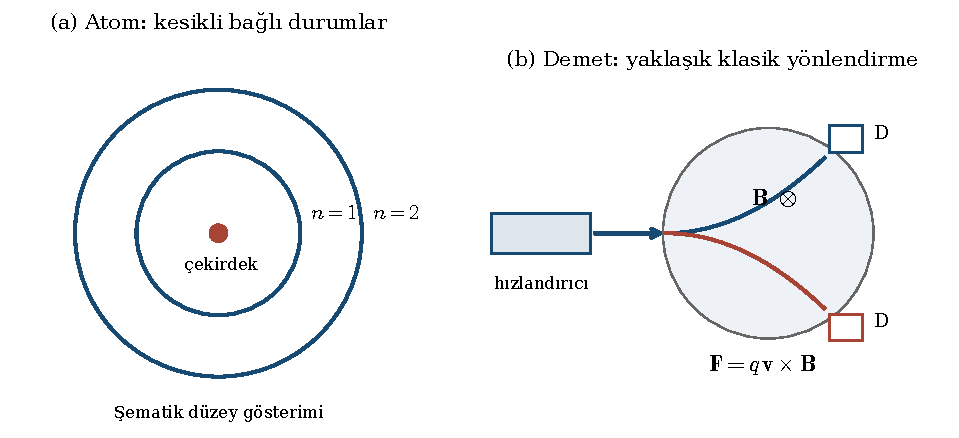
\includegraphics[width=\linewidth]{figurler/05_atom_demeti.pdf}
 \caption[Atomik durumlar ve parçacık demetleri]{Atomik bağlı durumlar ile bir parçacık demetinin yaklaşık
 klasik yönlendirilmesinin karşılaştırılması. Soldaki halkalar
 kesikli durumların şematik gösterimidir; elektronun gerçek yörüngesi
 olarak okunmamalıdır. Sağdaki eğriler farklı yük işaretleri için
 manyetik sapmayı, D kutuları dedektörleri simgeler.}
 \label{fig:05_atom_demeti}
\end{figure}

% Kaynak PDF s. 41--45: bölüm sonundaki momentum eki.
\subsection*{Ek: Momentum İşlemcisinin Hermitliği}
\phantomsection
\addcontentsline{toc}{subsection}{Ek: Momentum İşlemcisinin Hermitliği}
\label{sec:05_momentum_eki}

Momentum işlemcisinin Hermitliğini doğrudan gösterelim. Bu örnek
Hermit eşlenik ile kompleks eşlenik arasındaki farkı ve sınır
şartlarının rolünü de açıklar \cite[162--165]{book:Ficek}.

\subsubsection*{Beklenen değer ile matris elemanının ayrılması}

Aynı durumda alınan,
\begin{equation}
 \langle p\rangle_\psi=\int\psi^*(x)\hat p\psi(x)\,dx
\end{equation}
ifadesi beklenen değerdir. Buna karşılık iki farklı fonksiyonla
kurulan,
\begin{equation}
 \langle\phi|\hat p|\psi\rangle
 =\int\phi^*(x)\hat p\psi(x)\,dx
\end{equation}
bir \emph{matris elemanı}dır ve Hermit bir işlemci için bile genel
olarak reel olmak zorunda değildir. Hermitliğin gerektirdiği ilişki,
\begin{equation}
 \langle\phi|\hat p|\psi\rangle
 =\langle\psi|\hat p|\phi\rangle^*
\end{equation}
olur. Beklenen değerde $\phi=\psi$ seçildiği için reel sonuç elde
edilir.

\subsubsection*{Kısmi integrasyonla ispat}

$\hat p=-i\hbar\,d/dx$ için, $x_L<x<x_R$ aralığında,
\begin{align}
 \langle\phi|\hat p\psi\rangle
 &=-i\hbar\int_{x_L}^{x_R}\phi^*(x)\psi'(x)\,dx\\
 &=-i\hbar[\phi^*(x)\psi(x)]_{x_L}^{x_R}
   +i\hbar\int_{x_L}^{x_R}\phi'^*(x)\psi(x)\,dx\\
 &=-i\hbar[\phi^*\psi]_{x_L}^{x_R}
   +\langle\hat p\phi|\psi\rangle
 \label{eq:05_p_sinir_terimi}
\end{align}
bulunur. Dolayısıyla sınır terimi sıfırsa,
\begin{equation}
 \boxed{\langle\phi|\hat p\psi\rangle
       =\langle\hat p\phi|\psi\rangle}
 \label{eq:05_p_hermit_ic_carpim}
\end{equation}
sağlanır. Tam doğru üzerinde yeterince düzgün, kendisi ve türevi
kare integrallenebilir uygun fonksiyonlarla çalışıldığında,
$\hat p=-i\hbar d/dx$ için doğal kendine eşlenik tanım kümesi
kullanılabilir; sonsuzlardaki sınır katkısı yok olur.

Yalnızca $\psi$ ve $\phi$'nin kare integrallenebilir olduklarını
söylemek türevin varlığını, onun kare integrallenebilirliğini ve bütün
sınır işlemlerini tek başına garanti etmez. Bu nedenle momentumun
tanım kümesi dalga fonksiyonlarının uzayından daha dar seçilir.

Aynı hesabı eşlenik işlemciyi sol tarafa taşıyarak yazarsak,
\begin{align}
 \langle\phi|\hat p^\dagger\psi\rangle
 &=\langle\hat p\phi|\psi\rangle
 =i\hbar\int\phi'^*\psi\,dx\\
 &=i\hbar[\phi^*\psi]_{x_L}^{x_R}
   -i\hbar\int\phi^*\psi'\,dx.
\end{align}
Sınır terimi yokken türev ifadesi,
\begin{equation}
 \hat p^\dagger=-i\hbar\frac{d}{dx}=\hat p
\end{equation}
olur. Ancak tam işlemci eşitliği için tanım kümelerinin de
uyuşması gerekir. Sonlu aralıkta, örneğin,
\begin{equation}
 \psi(x_R)=e^{i\theta}\psi(x_L),\qquad
 \phi(x_R)=e^{i\theta}\phi(x_L)
\end{equation}
şeklinde aynı sabit $\theta$ ile verilen periyodik veya fazlı
periyodik koşullar, sınır teriminin yok olmasını ve uygun kendine
eşlenik momentum gerçekleşimini sağlar. İki uçta sıfır koşulu ise
momentumun simetrik olmasını sağlar ama tek başına kendine
eşlenikliğini sağlamaz. Sonsuz kuyu Hamiltonyeninin uygun sınır
şartları ile momentum işlemcisinin sınır şartları aynı soru değildir.

\subsubsection*{Kompleks eşlenik neden yeterli değildir?}

Yalnızca katsayıların kompleks eşleniği alındığında,
\begin{equation}
 \hat p^*=+i\hbar\frac{d}{dx}
\end{equation}
ifadesi elde edilir. Buna karşılık Hermit eşlenik alınırken kısmi
integrasyon türev işlemcisinden ek bir eksi işareti getirir. Bu
nedenle $\hat p^\dagger=\hat p$ olması ile
$\hat p^*=\hat p$ olması farklı iddialardır; momentum için ikincisi
geçerli değildir.

Bir ortonormal bazda momentumun matris elemanları,
\begin{equation}
 p_{jk}=\langle u_j|\hat p|u_k\rangle
\end{equation}
olarak tanımlanır. Hermitlik bu gösterimde,
\begin{equation}
 p_{jk}=p_{kj}^*,\qquad p=p^\dagger=(p^*)^{\mathsf T}
\end{equation}
şeklindedir. Örneğin Denk.~\eqref{eq:05_serbest_matrisler}'deki
momentum matrisi reel değildir; buna rağmen kompleks eşlenik
transpozu kendisine eşittir. Böylece diferansiyel gösterim, matris
gösterimi ve Dirac gösterimi aynı Hermitlik koşulunu ifade eder.

\BolumKaynakcaBitir
\end{document}
